\chapter{Tour d'horizon du prototype réalisé}
\label{AppendixA}

Le projet est disponible dans un dépôt publique hébergé chez \textit{GitHub}, à l'adresse : \textbf{\url{https://github.com/MichaelPolla/mip-viewer}}.

Sa racine est décomposée en trois répertoires :

\begin{itemize}
    \item \textbf{mip-viewer} : Code source du prototype.
    \item \textbf{project-report} : Rapport de projet (documents \LaTeX, images...).
    \item \textbf{sample-models} : Échantillons de modèles 3D pour tester le prototype.
\end{itemize}

\begin{figure}[h]
    \centering
    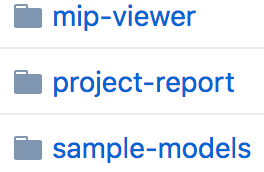
\includegraphics[height=0.1\linewidth]{Figures/mip-viewer-root-folder.png}
    \caption{Répertoires à la racine du projet.}
    \label{fig:mip-viewer-root-folder}
\end{figure}

\section{Instructions}
L'application peut rapidement être testée en suivant les instructions suivantes :
\begin{enumerate}
    \item Installer \textit{NodeJS}: \url{https://nodejs.org/}
    \item Cloner le projet: \texttt{git clone https://github.com/MichaelPolla/mip-viewer}
    \item Se placer dans le répertoire \texttt{mip-viewer} et exécuter :
    \begin{itemize}
        \item \texttt{npm install}
        \item \texttt{npm run dev}
    \end{itemize}
    \item L'outil est accessible dans le navigateur à l'adresse : \\ \url{http://localhost:3000/}.
    \item Glisser-déposer un répertoire contenant un modèle au format \textit{glTF}, tel que ceux proposés dans \texttt{sample-models} à l'emplacement indiqué.
    \item Ajouter une annotation en double-cliquant à l'endroit désiré.
\end{enumerate}

\section{Organisation du code}

\begin{figure}[h]
    \centering
    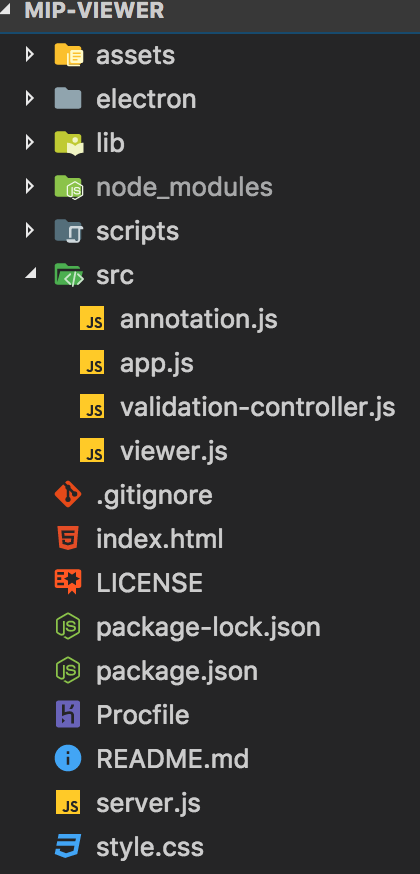
\includegraphics[width=0.25\linewidth]{Figures/mip-viewer-project-structure.png}
    \caption{Organisation du code du projet.}
    \label{fig:mip-viewer-project-structure}
\end{figure}

Le développeur qui souhaiterait continuer à développer ce projet s'intéressera particulièrement aux éléments suivants :

\begin{itemize}
    \item \texttt{package.json}: liste les dépendances du projet, et contient les scripts exécutés, par exemple, lorsque l'on exécute la commande `npm run dev`.
    \item \texttt{index.html}: définit les éléments web tel que la zone de \textit{drag-n-drop} de modèle, le canvas qui contiendra la visionneuse, ou encore le dialogue utilisé pour afficher et ajouter des annotations. Consulter également \texttt{style.css} pour la mise en forme.
    \item le répertoire \texttt{src} contient les fichiers \textit{JavaScript} principaux
    \begin{itemize}
        \item \texttt{app.js} est le point central du programme. Il gère la zone d'importation de modèles, le chargement des fichiers fournis par l'utilisateur puis la création de la visionneuse.
        \item \texttt{viewer.js} contient tout ce qui a trait à la visionneuse. La majorité du code du projet se trouve dans ce fichier. C'est par exemple ici qu'ont été ajoutés les événements liés à l'ajout et l'affichage des annotations.
        \item \texttt{annotation.js} enfin, définit la structure des annotations.
    \end{itemize}
\end{itemize}
